\documentclass[a4paper]{article}

\usepackage{/home/evasilyev/CLionProjects/algorithmic_foundation/settings}


\begin{document}

In this problem, a tree is an undirected graph that is connected and has no cycles.

The given input is a graph that started as a tree with $N$ nodes (with distinct values $1, 2, \dots, N$), with one additional edge added. The added edge has two different vertices chosen from $1$ to $N$, and was not an edge that already existed.

The resulting graph is given as a $2D$-array of edges. Each element of edges is a pair $[u, v]$ with $u < v$, that represents an undirected edge connecting nodes $u$ and $v$.

Return an edge that can be removed so that the resulting graph is a tree of $N$ nodes. If there are multiple answers, return the answer that occurs last in the given $2D$-array. The answer edge $[u, v]$ should be in the same format, with $u < v$.

\SPACE

\textbf{Example 1:}

\textbf{Input:} [[1,2],[1,3],[2,3]]

\textbf{Output:} [2,3]

\textbf{Explanation:} The given undirected graph will be like this:\\
\begin{center}
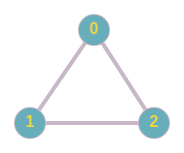
\includegraphics[width=3cm]{images/1.png}
\end{center}

\SPACE


\textbf{Example 2:}

\textbf{Input:} [[1,2], [2,3], [3,4], [1,4], [1,5]]

\textbf{Output:} [1,4]

\textbf{Explanation:} The given undirected graph will be like this:\\
\begin{center}
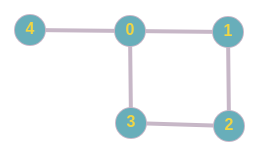
\includegraphics[width=5cm]{images/2.png}
\end{center}



\textbf{Note:}

\begin{itemize}
\item The size of the input $2D$-array will be between $3$ and $1000$
\item Every integer represented in the $2D$-array will be between $1$ and $N$, where $N$ is the size of the input array.
\end{itemize}








\end{document}
